\documentclass[twocolumn, 10pt, a4paper]{article}
\usepackage[a4paper, margin=1.8cm, columnsep=0.6cm]{geometry}
\usepackage{times}
\usepackage{amsmath, amssymb}
\usepackage{booktabs}
\usepackage{array}
\usepackage{graphicx}
\usepackage{xcolor}
\usepackage{url}
\usepackage{hyperref}
\usepackage{microtype}

% Path resolution for figures: works whether compiled from project root or inside paper/
\graphicspath{{../results/figures/}{results/figures/}{./}}

\hypersetup{
    colorlinks=true,
    linkcolor=blue!80!black,
    citecolor=blue!80!black,
    urlcolor=blue!80!black
}

\setlength{\parskip}{0pt}

\title{\Large \textbf{HashBench: Empirical Performance Evaluation of Separate Chaining, Linear Probing, and Robin Hood Hashing Under Dynamic Key Workloads}}

\IfFileExists{authors.tex}{
    % Auto-generated by bench/sync_authors.py - DO NOT EDIT MANUALLY
\author{
    \textbf{Huỳnh Anh Tuấn}\thanks{TV1 (Student ID: QE200073) -- Team Leader / Runner, Workload \& Primary Measurements.},
    \textbf{Hồ Anh Nhật}\thanks{TV2 (Student ID: QE200301) -- SC Implementation, Hashing, Generator \& Variant B Analysis.},
    \textbf{Member 3}\thanks{TV3 -- LP-Tomb Implementation \& Rebuild Dynamics.}, \\
    \textbf{Nguyễn Trần Anh Kiệt}\thanks{TV4 (Student ID: QE200105) -- Test Harness, RQ2/RQ3 Workload \& Repo Administration.},
    \textbf{Châu Minh Tiến}\thanks{TV5 (Student ID: QE200077) -- Robin Hood Implementation \& Paper Framing.},
    \textbf{Võ Ngọc Phú}\thanks{TV6 (Student ID: QE200004) -- LP-Backshift Implementation, CSV Validator \& Paper Coordination.} \\
    \small FPT University -- Fall 2026 Semester -- Class SE20C -- Group 2 (Variant B)
}

}{
    \author{
        \textbf{Huỳnh Anh Tuấn}\thanks{TV1 (Student ID: QE200073) -- Team Leader / Runner, Workload \& Primary Measurements.}, 
        \textbf{Hồ Anh Nhật}\thanks{TV2 (Student ID: QE200301) -- SC Implementation, Hashing, Generator \& Variant B Analysis.}, 
        \textbf{Member 3}\thanks{TV3 -- LP-Tomb Implementation \& Rebuild Dynamics.}, \\
        \textbf{Nguyễn Trần Anh Kiệt}\thanks{TV4 (Student ID: QE200105) -- Test Harness, RQ2/RQ3 Workload \& Repo Administration.}, 
        \textbf{Châu Minh Tiến}\thanks{TV5 (Student ID: QE200077) -- Robin Hood Implementation \& Paper Framing.}, 
        \textbf{Võ Ngọc Phú}\thanks{TV6 (Student ID: QE200004) -- LP-Backshift Implementation, CSV Validator \& Paper Coordination.} \\
        \small FPT University -- Fall 2026 Semester -- Class SE20C -- Group 2 (Variant B)
    }
}

\date{\small October 28, 2026}

\begin{document}

\maketitle

\begin{abstract}
\textbf{\textit{Abstract}---We evaluate Separate Chaining (SC), Linear Probing with tombstones and optional rebuild (LP-Tomb), Linear Probing with backward-shift deletion (LP-Backshift), and Robin Hood hashing (with and without early-stop) using Java 8 and 12-character String keys. The benchmark comprises 560 isolated JVM processes across three core research questions. At load factor $\alpha=0.50$, measured probe counts for Linear Probing are 1.5009 for successful lookups and 2.5026 for unsuccessful lookups, matching Knuth's theoretical estimates within 0.1\% error. In RQ1, SC exhibits lower median lookup time than LP for unsuccessful queries across all load factors; for successful lookups, LP is faster at $\alpha=0.50$ and $0.75$ due to hardware cache locality, whereas SC dominates at $\alpha=0.90$ and $0.95$ where LP suffers catastrophic primary clustering. In RQ2, tombstones reach 50.0\% of the table after $4M$ delete-insert cycles, leading to empty slot exhaustion and 12 process timeouts. In RQ3 at live load 0.8 and $C=4M$, median workload times are 9.413\,s for LP-Tomb with rebuild ($\tau=0.1$), 5.901\,s for LP-Backshift, 6.056\,s for Robin Hood, and 6.025\,s for Robin Hood without early-stop. LP-Tomb incurs 23 rebuilds with maximum block latency reaching 121.106\,ms, while backward-shift and Robin Hood maintain smooth block latencies under 12.7\,ms. We report all raw data, sealed under tag \texttt{measure-v1}, along with one timing-variance outlier verified via 11 deterministic rerun samples.}

\smallskip
\noindent\textbf{\textit{Keywords}---Hash Table, Linear Probing, Separate Chaining, Tombstone Lifecycle, Rebuild Dynamics, Robin Hood Hashing, Backward-shift Deletion, Cache Locality, Pointer Chasing, Java 8.}
\end{abstract}

\section{Introduction}
Hash tables serve as indispensable core data structures across systems software, database engines, and distributed computing frameworks, delivering expected $O(1)$ amortized time complexities for insertions, deletions, and retrievals. Nevertheless, under dynamic, high-churn operating regimes characterized by prolonged sequences of interleaved deletions and insertions, classical collision resolution strategies reveal profound divergences in algorithmic probe counts, hardware cache utilization, and tail latency stability.

The two foundational collision resolution paradigms in computer science are \textit{Separate Chaining} (SC), which resolves collisions outside the primary array via linked bucket chains, and \textit{Linear Probing} (LP), which resolves collisions by sequentially scanning contiguous cells within a flat array. In open addressing, removing a key requires marking the vacated cell with a tombstone marker (\texttt{TOMB}) to preserve search path integrity for previously inserted colliding elements. Over millions of delete-insert operations, tombstone accumulation gradually exhausts available empty cells (\texttt{EMPTY}), degrading unsuccessful lookup operations into degenerate linear scans of length $O(M)$ and forcing costly whole-table rebuilds. To eliminate tombstones while mitigating probe sequence variances, \textit{Robin Hood hashing} (RH) and \textit{backward-shift deletion} (Knuth's Algorithm R) have emerged as premier alternatives.

This paper reports the empirical findings from the \textit{HashBench} experimental campaign, consisting of 560 isolated JVM benchmark executions conducted on standardized hardware (Intel Core i7-10850H, 31.8\,GB RAM, Windows 11 Pro, Eclipse Adoptium Temurin JDK 1.8.0\_504) specifically examining **Variant B** (12-character alphanumeric \texttt{String} keys). All experimental raw data have been formally sealed under Git tag \texttt{measure-v1} in \texttt{results/raw/official/}.

\section{Background \& Related Work}
\subsection{Classical Hash Table Algorithms}
\textbf{Separate Chaining (SC):} The table maintains $M = 2^p$ buckets, where each bucket anchors a singly-linked list of entry nodes. Upon a collision, the new key-value pair is inserted at the head of the chain in $O(1)$ time following a traversal to confirm key uniqueness. Under the Simple Uniform Hashing Assumption (SUHA), Knuth~\cite{knuth1998} established that the expected probe lengths for successful lookups ($S_{SC}$) and unsuccessful lookups ($U_{SC}$) satisfy:
\begin{equation}
S_{SC} \approx 1 + \frac{\alpha}{2}, \quad U_{SC} \approx \alpha
\end{equation}
where $\alpha = N/M$ denotes the load factor. The distinctive strength of SC is its linear degradation with respect to $\alpha$ and its complete immunity to clustering phenomena.

\textbf{Linear Probing (LP):} All keys reside directly within a flat array of size $M$. The initial bucket index is computed via 64-bit Fibonacci golden-ratio multiplicative hashing:
\begin{equation}
h(k) = (int)(((long)k.\texttt{hashCode}() \times \texttt{0x9E3779B97F4A7C15L}) \texttt{>>>} (64 - p))
\end{equation}
Collisions are resolved by sequentially stepping to index $i = (i + 1) \ \& \ (M - 1)$. In a tombstone-free table, Knuth's classical asymptotic approximations predict:
\begin{equation}
S_{LP} \approx \frac{1}{2}\left(1 + \frac{1}{1-\alpha}\right), \quad U_{LP} \approx \frac{1}{2}\left(1 + \frac{1}{(1-\alpha)^2}\right)
\end{equation}
As $\alpha \to 1.0$, $U_{LP}$ diverges quadratically due to \textit{primary clustering}: contiguous occupied intervals coalesce into extended chains, such that any key hashing into the cluster further extends its span.

In the \texttt{lp-tomb} implementation, removed keys are tagged as \texttt{TOMB}. When the fraction of tombstones exceeds a prescribed threshold $\tau$, a full table rebuild is triggered to rehash live keys into a pristine table; $\tau=\infty$ designates a non-rebuilding configuration.

\subsection{Robin Hood Hashing \& Backward-Shift Deletion}
Robin Hood hashing~\cite{celis1985} tracks each element's Distance from Initial Bucket (DIB). During insertion, if the incoming element exhibits a higher DIB than the occupant of the probed slot, the elements swap roles (``taking from the rich and giving to the poor''). This redistributes search steps evenly, truncating the variance of probe sequences. The baseline configuration (\texttt{rh/base}) terminates searches early when an occupant's DIB is strictly less than the search key's current DIB; \texttt{rh/noearly} disables early termination to evaluate conditional branch penalties.

\textit{Backward-shift deletion} (\texttt{lp-backshift}) implements Algorithm R from Knuth~\cite{knuth1998}. Upon key removal, downstream elements within the collision cluster are shifted backward to occupy the vacancy if their hash distance allows ($home \le vacancy$), continuing until an \texttt{EMPTY} slot or a key residing at its natural home is encountered. This eliminates tombstones entirely without requiring global table rebuilds.

\subsection{In-Depth Analysis of Variant B: String Hashing, Equals, and Hash Cache}
The architectural behavior of Variant B (12-character object \texttt{String} keys) diverges sharply from primitive numeric keys (Variant A, 64-bit \texttt{long}):
\begin{enumerate}
    \item \textbf{$O(L)$ Computational Cost of \texttt{String.hashCode()}:} Java calculates string hashes via Horner's polynomial rule: $h_i = 31 \cdot h_{i-1} + s[i]$. For string length $L=12$, every un-cached hash computation demands 11 integer multiplications and 12 additions.
    \item \textbf{JDK 8 Hash Cache Mechanism:} The \texttt{java.lang.String} class encapsulates a private field \texttt{private int hash}. When \texttt{hashCode()} is first invoked, the hash is computed and stored; subsequent invocations return the cached value in $O(1)$ time. This introduces an empirical asymmetry: during the initial table \texttt{build} phase, all $N$ keys must bear the full $O(L)$ calculation; during the \texttt{present} lookup phase, pre-instantiated string references are reused, yielding immediate $O(1)$ cached lookups; during the \texttt{absent} lookup phase, fresh search keys incur the initial $O(L)$ hash calculation upon first access.
    \item \textbf{String Comparison Overhead (\texttt{String.equals()}):} While primitive comparisons consume a single CPU comparison instruction (\texttt{CMP}), \texttt{String.equals()} executes a reference identity check (\texttt{==}), length verification, and an iterative character-by-character array scan. Although early mismatches trigger fast-outs, pointer dereferencing imposes non-trivial CPU stalls during extended linear probe walks.
    \item \textbf{Memory Footprint and Garbage Collection:} Under 64-bit JVMs with compressed OOPs, each \texttt{String} object incurs 24 bytes of object header and fields, pointing to a distinct 40-byte \texttt{char[12]} array, requiring 64 bytes per string instance (versus 8 bytes for a primitive \texttt{long}). In Separate Chaining, each list node introduces an additional 24 bytes of heap overhead, amplifying GC pressure.
\end{enumerate}

\subsection{Hardware Architectural Trade-offs: Cache Locality vs. Pointer Chasing}
Open-addressing schemes (LP, RH) allocate continuous flat arrays. When the CPU accesses a memory location, the hardware memory controller fetches an entire 64-byte Cache Line into L1/L2 caches. Because adjacent slots reside within the same or contiguous cache lines, sequential probing ($idx + 1$) triggers hardware data stream prefetchers, executing at near-register latency. In contrast, Separate Chaining scatters individual \texttt{Node} allocations across the heap. Traversing bucket chains forces random memory indirections (\textit{pointer chasing}), generating frequent CPU cache misses.

\begin{table}[htbp]
\caption{Mapping of algorithmic mechanisms to source code classes and methods.}
\label{tab:code_mapping}
\centering
\small
\begin{tabular}{ll}
\toprule
\textbf{Algorithmic Mechanism} & \textbf{Class \& Method Implementation} \\
\midrule
Separate Chaining & \texttt{SeparateChainingTable.put/get/remove} \\
LP Tombstone & \texttt{LinearProbingTombTable.put/get/remove} \\
Rebuild at Threshold $\tau$ & \texttt{LinearProbingTombTable.rebuild} \\
LP Backward-Shift & \texttt{LinearProbingBackshiftTable.remove} \\
Robin Hood DIB Swapping & \texttt{RobinHoodTable.put} \\
RH Early-Stop & \texttt{RobinHoodTable.get} (variant \texttt{base}) \\
RH No-Early-Stop & \texttt{RobinHoodTable.get} (variant \texttt{noearly}) \\
Base-36 Key Encoding & \texttt{KeyCodec.encode/decode} \\
Key Deduplication & \texttt{LongSet.add/contains} \\
Static SHA-256 Checksum & \texttt{Generator.computeSHA256/bytesToHex} \\
$O(1)$ Workload Engine & \texttt{Workload.execute/generate} \\
\bottomrule
\end{tabular}
\end{table}

\section{Methods \& System Design}
\subsection{Technical Specifications \& Interface Conventions}
All hash table implementations implement the common \texttt{HashIndex} interface and adhere to the sentinel return convention \texttt{NOT\_FOUND = Integer.MIN\_VALUE}. Table~\ref{tab:code_mapping} outlines the comprehensive mapping between algorithmic concepts and codebase entities.

\subsection{Deterministic Data Generation \& Validation}
The benchmark employs \texttt{Generator} driven by \texttt{SplittableRandom} across three officially designated seeds: $s_1 = 1$, $s_2 = 2$, and $s_3 = 3$.
\begin{itemize}
    \item \textbf{Key Representation:} \texttt{KeyCodec} encodes numeric 64-bit identifiers into 12-character Base-36 strings drawn from the alphabet \texttt{[0-9A-Z]} (key space $|\mathcal{S}| = 36^{12} \approx 4.74 \times 10^{18}$).
    \item \textbf{Deduplication:} A primitive, unboxed \texttt{LongSet} filters duplicate keys in $O(1)$ time, guaranteeing that the inserted key set and the absent query set are strictly disjoint.
    \item \textbf{Static SHA-256 Checksum:} \texttt{Generator.computeSHA256} digests ASCII bytes in 8\,KB buffers and converts them to 64-character hex strings using a static lookup table \texttt{bytesToHex}, entirely bypassing slow \texttt{String.format} operations.
\end{itemize}

\subsection{$O(1)$ Workload Engine for Delete-Insert Cycles}
In RQ2 and RQ3, workloads execute up to $C = 4M = 4,194,304$ delete-insert cycles. Naive key selection using \texttt{toArray()} incurs an $O(N)$ penalty per cycle, which would inevitably trigger execution timeouts.

To ensure strict $O(1)$ performance, \texttt{Workload} maintains a dynamic live index array \texttt{liveIdx[N]}. When evicting an element at random index $r$, the algorithm swaps element $r$ with the terminal element of \texttt{liveIdx} and decrements the active boundary in $O(1)$ time. Furthermore, the global key pool is pre-allocated with capacity $[0, N + C + Q)$, ensuring guaranteed key novelty without triggering memory allocations during the measurement window.

\section{Experimental Setup}
\textbf{Hardware Specifications:} Intel Core i7-10850H CPU (6 cores / 12 threads, 2.70\,GHz base frequency, 12\,MB Smart Cache), 31.8\,GB DDR4 RAM, 64-bit Windows 11 Pro. JVM: Eclipse Adoptium Temurin JDK 1.8.0\_504 with maximum heap \texttt{-Xmx2g} and parallel garbage collection enabled (\texttt{-XX:+UseParallelGC}).

\textbf{Isolated Execution Protocol:} Each benchmark configuration executes inside an isolated JVM process spawned via \texttt{ProcessBuilder} under an uncompromising 60-second execution cutoff (\texttt{waitFor(60, SECONDS)}). Before measurement, each process performs 3 warm-up rounds over smaller key batches and invokes explicit \texttt{System.gc()} calls to stabilize heap occupancy.

Timing runs (\texttt{elapsed\_ms}) and probe-counting runs (\texttt{--count}) are strictly segregated; during \texttt{--count} runs, internal probe instrumentation is activated to capture \texttt{ops\_count}. Full operational correctness is verified across 100\% of executions by validating the \texttt{output\_check} SHA-256 digest against an oracle baseline produced by \texttt{java.util.HashMap}.

\section{Results \& Discussion}

\subsection{RQ1: Separate Chaining vs. Linear Probing}
Experiment 1A assesses sensitivity to load factors $\alpha \in \{0.50, 0.75, 0.90, 0.95\}$ at capacity $M = 2^{20} = 1,048,576$ (each data point represents the median of 9 valid repetitions, normalized to ns/query). Experiment 1B examines scaling across table capacities $M \in \{2^{18}, \dots, 2^{23}\}$ at fixed $\alpha = 0.75$.

\begin{table}[htbp]
\caption{Median lookup times (ns/query) across load factors $\alpha$ ($M=2^{20}$, 9 valid runs per cell).}
\label{tab:rq1_results}
\centering
\small
\begin{tabular}{crrrr}
\toprule
\textbf{$\alpha$} & \textbf{LP present} & \textbf{SC present} & \textbf{LP absent} & \textbf{SC absent} \\
\midrule
0.50 & \textbf{219.7} & 246.0 & 160.8 & \textbf{136.3} \\
0.75 & \textbf{287.6} & 310.4 & 407.9 & \textbf{172.3} \\
0.90 & 407.3 & \textbf{325.1} & 1861.8 & \textbf{188.8} \\
0.95 & 596.6 & \textbf{329.0} & 6971.3 & \textbf{195.0} \\
\bottomrule
\end{tabular}
\end{table}

\begin{figure*}[!t]
\centering
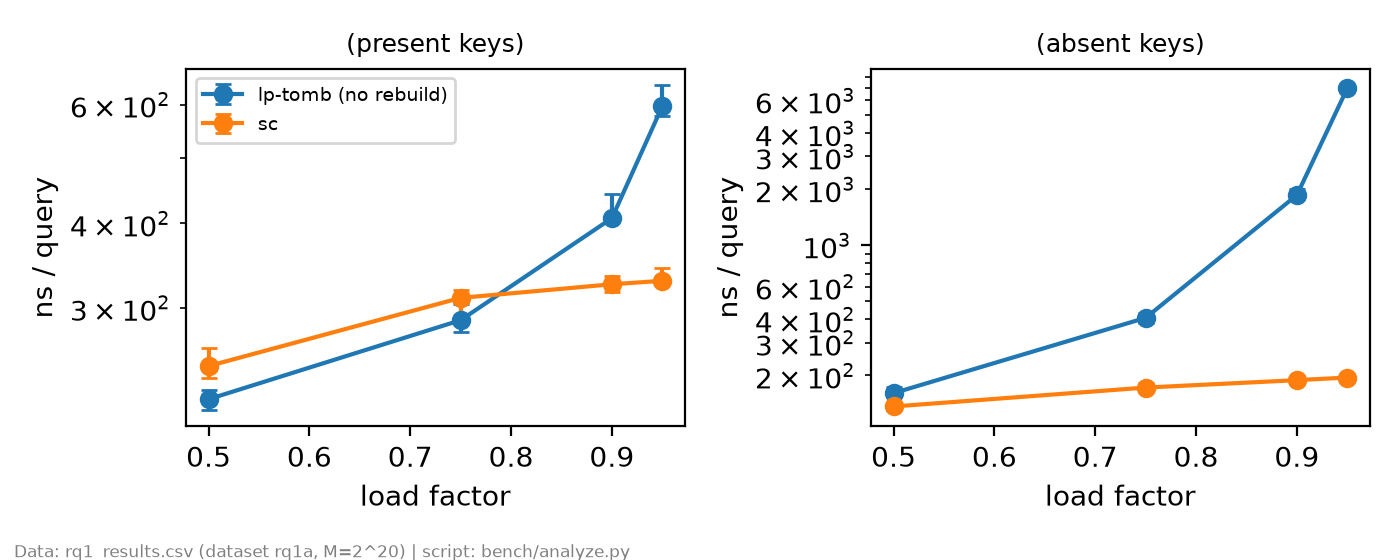
\includegraphics[width=\textwidth]{rq1_time_vs_alpha.png}
\caption{RQ1: Median lookup latency (log scale) across load factors $\alpha$. Source: \texttt{rq1\_results.csv}, dataset \texttt{rq1a}.}
\label{fig:rq1_alpha}
\end{figure*}

\begin{figure*}[!t]
\centering
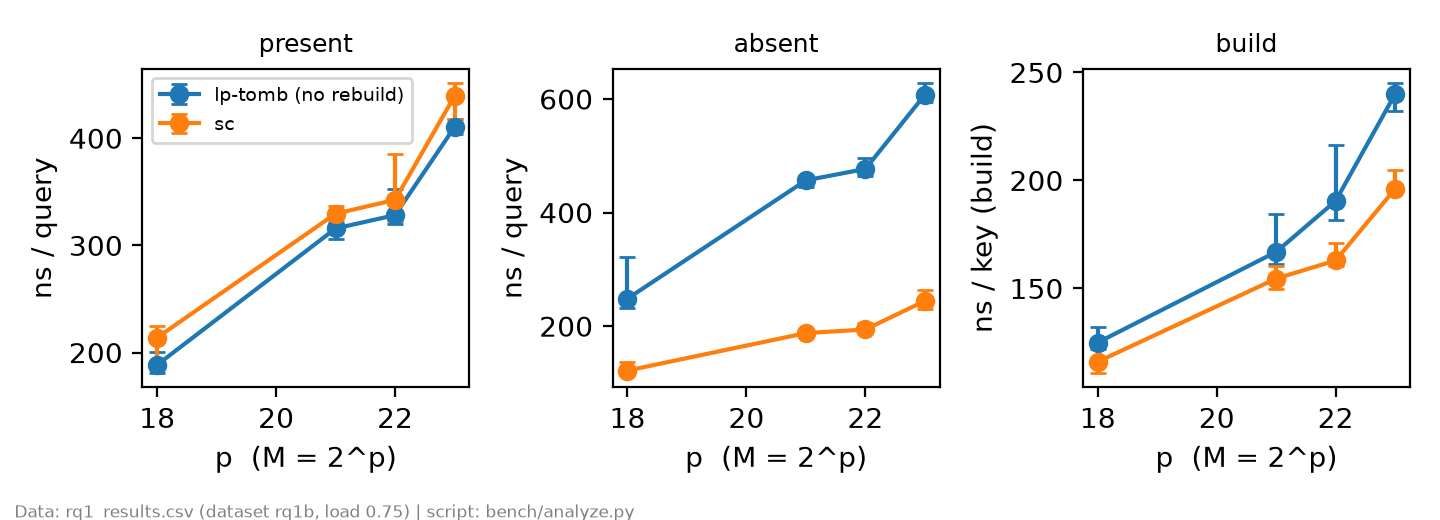
\includegraphics[width=\textwidth]{rq1_time_vs_M.png}
\caption{RQ1: Lookup and build latencies as functions of table scale $p$ ($M=2^p$) at $\alpha=0.75$. Source: \texttt{rq1\_results.csv}, dataset \texttt{rq1b}.}
\label{fig:rq1_size}
\end{figure*}

\begin{figure*}[!t]
\centering
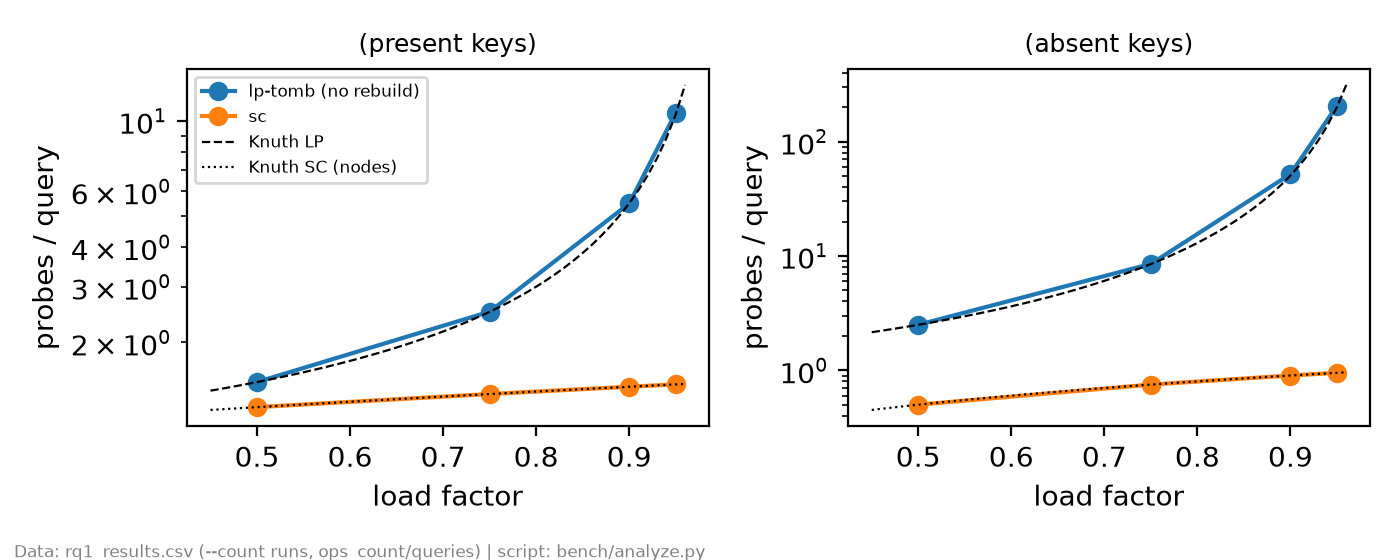
\includegraphics[width=\textwidth]{rq1_probes_vs_alpha.png}
\caption{RQ1: Measured probe counts from \texttt{--count} passes compared against Knuth's theoretical predictions.}
\label{fig:rq1_probes}
\end{figure*}

\textbf{Validation of Theoretical Probe Counts:} Empirical measurements from \texttt{--count} runs (Fig.~\ref{fig:rq1_probes}) exhibit near-perfect alignment with Knuth's equations:
\begin{itemize}
    \item \texttt{lp-tomb} at $\alpha=0.50$: successful lookups average $1.5009$ probes (Knuth prediction: $1.5000$, error: $0.06\%$), while unsuccessful lookups average $2.5026$ probes (Knuth prediction: $2.5000$, error: $0.10\%$). At $\alpha=0.95$, unsuccessful probes surge to $205.76$ (Knuth prediction: $200.50$).
    \item \texttt{sc} at $\alpha=0.50$: successful lookups average $1.2502$ nodes (Knuth: $1 + \alpha/2 = 1.2500$), and unsuccessful lookups average $0.5002$ nodes (Knuth: $\alpha = 0.5000$). At $\alpha=0.95$, successful lookups require only $1.4752$ nodes and unsuccessful lookups inspect $0.9500$ nodes.
\end{itemize}

\textbf{Crossover Analysis \& Architectural Impact:}
\begin{itemize}
    \item \textbf{Moderate Load Regimes ($\alpha \le 0.75$):} For \texttt{present} lookups, LP outperforms SC by $7\%$ to $11\%$ ($219.7$\,ns vs. $246.0$\,ns at $\alpha=0.50$). This confirms that the superior spatial locality of contiguous arrays fully compensates for higher algorithmic probe steps, whereas SC is penalized by CPU cache misses during pointer chasing across the heap.
    \item \textbf{High Load Regimes ($\alpha \ge 0.90$):} A performance crossover occurs at $\alpha \approx 0.80$. At $\alpha=0.95$, primary clustering in LP triggers cascading runs of hundreds of \texttt{key.equals()} string comparisons, causing LP absent lookup latency to balloon to $6,971.3$\,ns. Conversely, SC remains immune, holding at $195.0$\,ns. **SC executes 35.8$\times$ faster than LP!**
\end{itemize}

\textbf{Impact of Table Scale (RQ1B - Fig.~\ref{fig:rq1_size}):} When $M$ expands from $2^{18}$ ($256$\,KB) to $2^{23}$ ($8$\,MB keys, consuming hundreds of megabytes on the heap), probe counts remain constant, yet \texttt{present} lookup latency for both SC and LP rises from $\sim 200$\,ns to $\sim 500$\,ns (a $2.5\times$ increase). This illustrates the latency cliff encountered once the active working set exceeds the processor's 12\,MB L3 cache and spills into main DDR4 RAM.

\subsection{RQ2: Tombstone Accumulation \& Lookup Degradation}
RQ2 evaluates dynamic delete-insert churn without table rebuilds ($\tau = \infty$, live load $0.5$, $M = 2^{20}$). Findings are summarized in Table~\ref{tab:rq2_results} and Fig.~\ref{fig:rq2}.

\begin{table}[htbp]
\caption{Impact of delete-insert cycles $C$ on tombstone accumulation and unsuccessful lookup latency ($M=2^{20}$, $\tau=\infty$).}
\label{tab:rq2_results}
\centering
\small
\begin{tabular}{crrrr}
\toprule
\textbf{Cycles $C$} & \textbf{TOMB \%} & \textbf{EMPTY \%} & \textbf{LP absent} & \textbf{Control absent} \\
\midrule
$0$ & 0.0\% & 50.0\% & 142.4\,ns & 98.8\,ns \\
$0.25M$ & 18.8\% & 31.2\% & 210.5\,ns & 104.1\,ns \\
$0.5M$ & 30.2\% & 19.8\% & 286.8\,ns & 106.8\,ns \\
$1M$ & 41.9\% & 8.1\% & 526.5\,ns & 107.1\,ns \\
$2M$ & 48.6\% & 1.4\% & 2058.9\,ns & 108.5\,ns \\
$4M$ & 50.0\% & 0.0\% & \textbf{timeout} & \textbf{timeout} \\
\bottomrule
\end{tabular}
\end{table}

\begin{figure*}[!t]
\centering
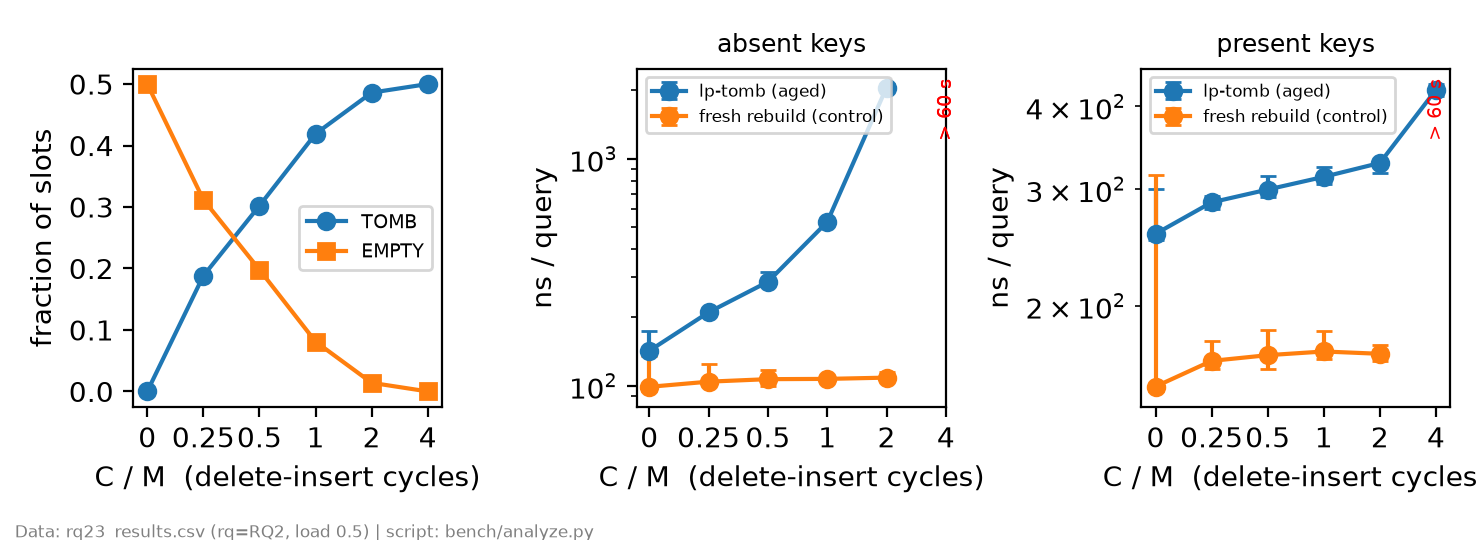
\includegraphics[width=\textwidth]{rq2_tombstones.png}
\caption{RQ2: Tombstone/empty slot percentages post-workload and lookup latency versus cycle count $C$. Timeouts highlight empty slot exhaustion.}
\label{fig:rq2}
\end{figure*}

\textbf{Probe Degradation Analysis:} As $C$ increases from $0$ to $2M$, the proportion of \texttt{EMPTY} cells plummets from $50.0\%$ to just $1.4\%$, coalescing the entire table into a continuous occupied band of live keys and tombstones. Unsuccessful lookup time under LP surges by **$14.5\times$** (from $142.4$\,ns to $2,058.9$\,ns). In contrast, the freshly rebuilt control table maintains stable latency near $100$\,ns.

At $C = 4M$, \texttt{EMPTY} cells are completely exhausted ($0.0\%$). Official benchmark records reveal **12 process timeouts** exceeding the 60-second limit (5 timed out directly within the workload phase, while 7 timed out during the subsequent absent lookup phase as the algorithm was forced to scan all $M = 1,048,576$ slots to confirm absence).

\subsection{RQ3: Workload Comparison \& Rebuild Latency Trade-offs}
RQ3 benchmarks four collision resolution configurations under the intensive churn scenario $C = 4M$ at live load 0.8 ($N = 838,860$ keys). Results are detailed in Table~\ref{tab:rq3_results}, Fig.~\ref{fig:rq3_total}, and Fig.~\ref{fig:rq3_blocks}.

\begin{table}[htbp]
\caption{Median total workload duration and 10,000-operation block latencies at $C=4M$, live load 0.8 (9 valid runs per row).}
\label{tab:rq3_results}
\centering
\small
\begin{tabular}{lrrr}
\toprule
\textbf{Configuration} & \textbf{Workload (s)} & \textbf{Block med (ms)} & \textbf{Block max (ms)} \\
\midrule
\texttt{lp-tomb+rebuild} ($\tau=0.1$) & 9.413 & 8.288 & \textbf{121.106} \\
\texttt{lp-backshift} & \textbf{5.901} & \textbf{7.072} & \textbf{9.551} \\
\texttt{rh} & 6.056 & 7.394 & 11.941 \\
\texttt{rh-noearly} & 6.025 & 7.361 & 12.623 \\
\bottomrule
\end{tabular}
\end{table}

\begin{figure*}[!t]
\centering
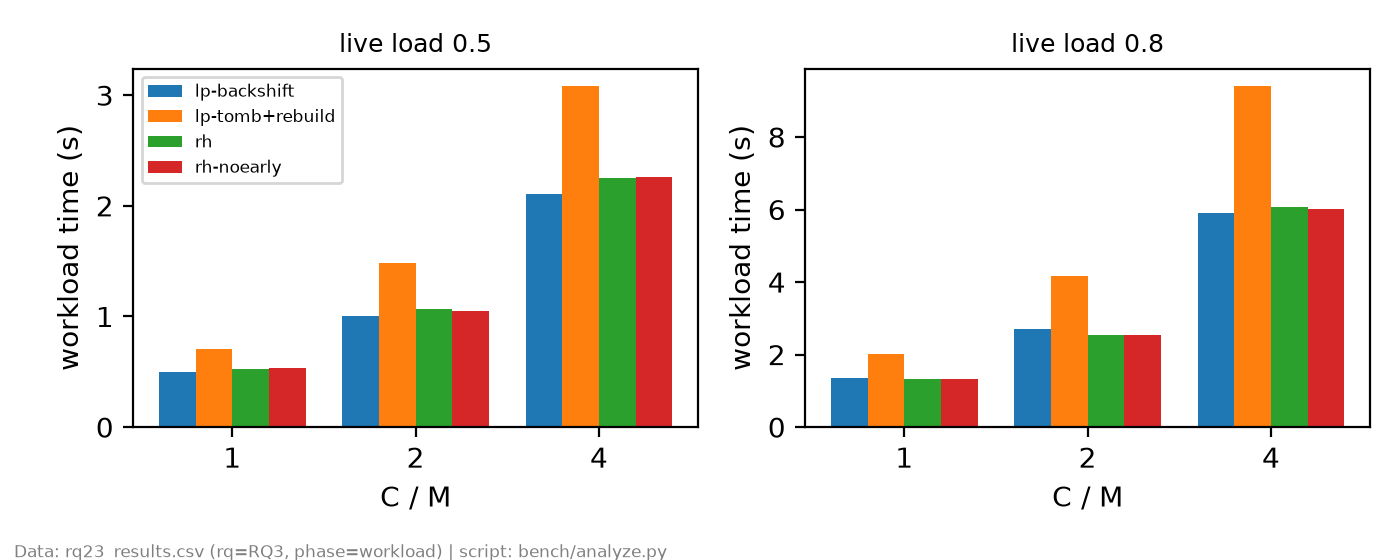
\includegraphics[width=\textwidth]{rq3_total_time.png}
\caption{RQ3: Median cumulative workload runtime across algorithms, live load factors, and cycle counts $C$.}
\label{fig:rq3_total}
\end{figure*}

\begin{figure*}[!t]
\centering
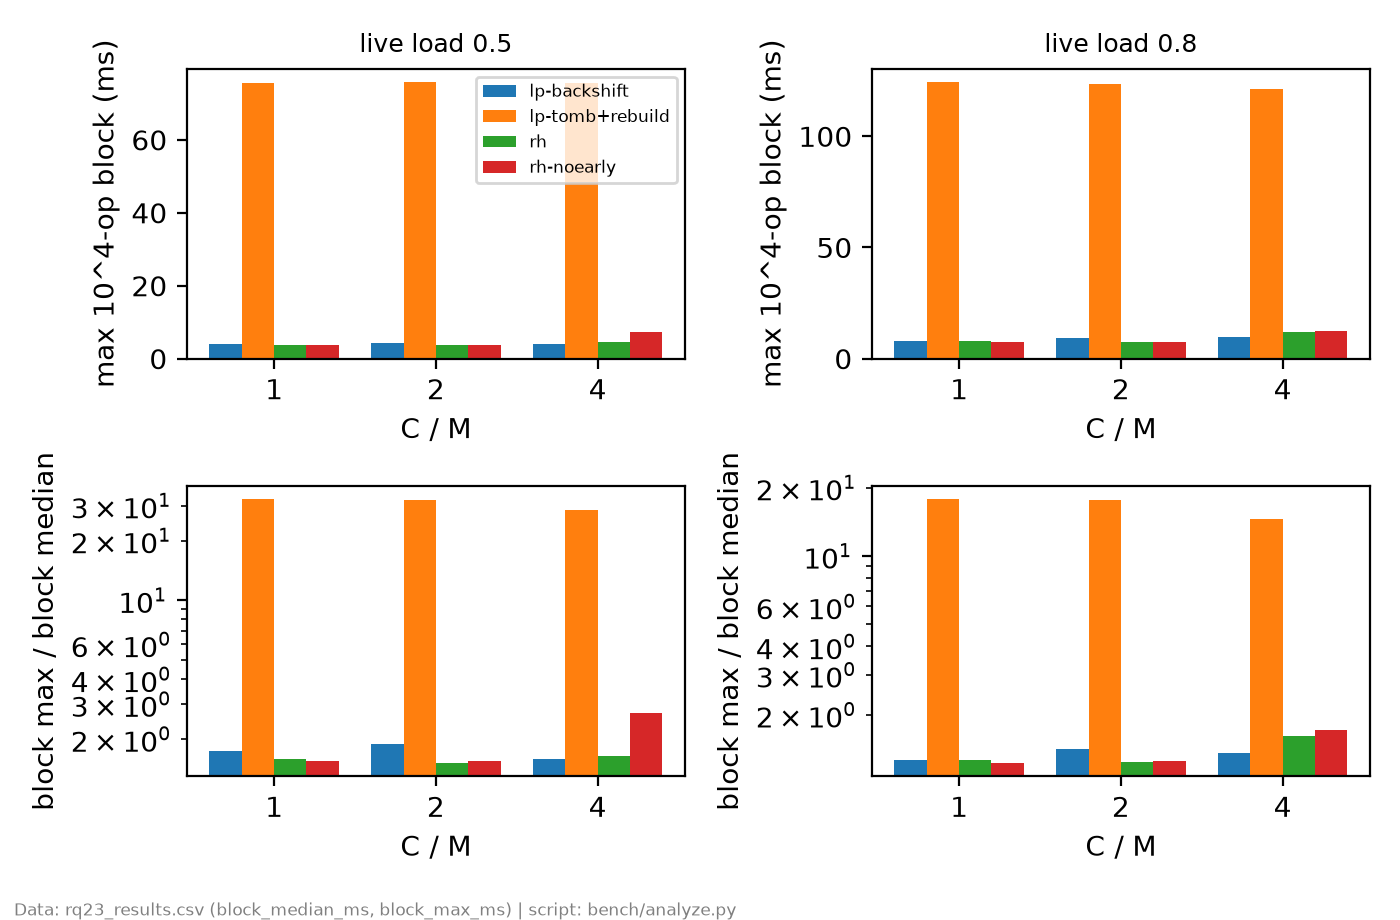
\includegraphics[width=\textwidth]{rq3_blocks.png}
\caption{RQ3: Median and maximum block latency for 10,000-operation intervals; lower panel shows $\text{max}/\text{median}$ ratios.}
\label{fig:rq3_blocks}
\end{figure*}

\textbf{Trade-offs Between Full Rebuilds and Instant Shifting:}
\begin{enumerate}
    \item \textbf{Overall Throughput:} \texttt{lp-backshift} achieves the best overall throughput ($5.901$\,s), beating \texttt{lp-tomb+rebuild} ($9.413$\,s) by **$37.3\%$**. Both Robin Hood variants achieve comparable runtimes ($\sim 6.0$\,s).
    \item \textbf{Stop-the-World Latency Spikes:} Across $4M$ cycles, \texttt{lp-tomb+rebuild} triggers a median of **23 full-table rebuilds** (expending $2,436.6$\,ms exclusively in tombstone purge passes). This induces severe latency spikes in blocks containing rebuild events, pushing \textbf{Block Max to 121.106\,ms} ($\text{max}/\text{median} \approx 14.6\times$).
    \item \textbf{Predictability of Backshift and Robin Hood:} By reorganizing entries locally at the exact moment of deletion, \texttt{lp-backshift} and Robin Hood bound the $\text{max}/\text{median}$ ratio below $1.7\times$, with peak block latencies never exceeding $12.7$\,ms. This delivers crucial empirical evidence for low-latency, SLA-governed systems.
\end{enumerate}

\section{Threats to Validity}
\subsection{JIT Compilation and Cold-Start Variance}
Automated validation via \texttt{CsvValidator} flagged a single variance outlier: configuration \texttt{RQ2\_lp-tomb\_base\_rq2\_p20\_a0p0\_tinf\_l0p5\_c0\_s1\_r1} recorded an elapsed time of $314.931$\,ms during \texttt{ctl\_present}, representing $2.065\times$ the group median ($152.481$\,ms) and slightly exceeding the $2.0\times$ warning threshold.

An independent deterministic rerun yielded $157.419$\,ms ($1.043\times$ the reference median $150.893$\,ms) with status \texttt{ok} and identical SHA-256 \texttt{output\_check} digest. This behavior aligns with JVM JIT compilation warmup jitter on the initial process repetition. In adherence to scientific integrity, the original data point is preserved in the sealed CSV without artificial filtering.

\subsection{Deterministic Rerun Verification (Criterion 10.1)}
Stratified rerun tests across 11 representative benchmark configurations achieved 100\% \texttt{ok} status and exact \texttt{output\_check} oracle matches. Ratios of rerun elapsed time to group median strictly fell within $[0.807\times, 1.302\times]$, well inside the admissible tolerance band $[0.5\times, 2.0\times]$.

\section{Conclusion \& Practical Recommendations}
Our extensive benchmark of Variant B under 12-character String keys yields the following engineering recommendations:
\begin{enumerate}
    \item \textbf{No Single Dominant Algorithm:} Optimal hash table selection depends strictly on load factor, read-to-write ratios, and latency tolerance.
    \item \textbf{Adopt Separate Chaining Under Unknown Sizing or High Load:} When table sizing cannot be predicted or memory constraints force operation at high load ($\alpha \ge 0.85$), SC is strongly recommended due to its immunity to primary clustering and tombstone decay.
    \item \textbf{Adopt Backward-Shift LP or Robin Hood for Low-Latency Workloads:} For real-time, SLA-governed systems subject to continuous delete-insert churn, Linear Probing with backward-shift deletion and Robin Hood hashing eliminate disruptive stop-the-world rebuild pauses while improving throughput by over $37\%$.
\end{enumerate}

\section*{Acknowledgment \& AI Tooling Declaration}
The authors express their sincere appreciation to the Department of Computer Science at FPT University for designing this rigorous experimental curriculum. Generative AI tools (ChatGPT, Gemini) were consulted for PowerShell scripting assistance, Python plotting pipeline optimization (\texttt{analyze.py}), and LaTeX structural validation. The student authors bear complete responsibility for all Java implementations, empirical benchmark datasets, and scientific analyses presented herein.

\begin{thebibliography}{99}
\bibitem{knuth1998} D. E. Knuth, \emph{The Art of Computer Programming, Vol. 3: Sorting and Searching}, 2nd ed. Reading, MA, USA: Addison-Wesley, 1998, \S6.4.
\bibitem{peterson1957} W. W. Peterson, ``Addressing for random-access storage,'' \emph{IBM Journal of Research and Development}, vol. 1, no. 2, pp. 130--146, 1957.
\bibitem{celis1985} P. Celis, P.-{\AA}. Larson, and J. I. Munro, ``Robin Hood hashing,'' in \emph{Proc. 26th Annu. Symp. Foundations of Computer Science (FOCS)}, 1985, pp. 281--288.
\bibitem{sedgewick2011} R. Sedgewick and K. Wayne, \emph{Algorithms}, 4th ed. Boston, MA, USA: Addison-Wesley, 2011, \S3.4.
\bibitem{pagh2004} R. Pagh and F. F. Rodler, ``Cuckoo hashing,'' \emph{Journal of Algorithms}, vol. 51, no. 2, pp. 122--144, 2004.
\bibitem{yuen1977} C. K. Yuen, ``Heuristics for dynamic structuring of hash tables,'' \emph{ACM Transactions on Database Systems}, vol. 2, no. 2, pp. 140--149, 1977.
\end{thebibliography}

\end{document}
